\documentclass[UTF8]{ctexart}
\usepackage{amsmath}
\usepackage{diagbox}
\usepackage{amsfonts}
\usepackage{textcomp}
\usepackage{graphicx}
\usepackage{float}
\usepackage{caption}
\usepackage{adjustbox}
\usepackage{subfigure}
\usepackage{geometry}
\usepackage{pifont}
\usepackage{gensymb}
\usepackage{bm}

\begin{document}
\renewcommand{\thefootnote}{\fnsymbol{footnote}}
\newgeometry{left=2cm,bottom=4cm,right=2cm}
\linespread{1.4}
\title{\vspace{-5em}\heiti电磁波在同轴电缆传输线中的传输特性实验报告\vspace{-2.5em}}
\date{}
\maketitle
\begin{center}
{\fangsong 徐浩博\quad 软件02\quad2020010108}
\end{center}

\subsubsection*{摘要}
{\kaishu\normalsize   本实验主要通过理论推导,实验测试和现象观察,对高频电磁波在同轴电缆传输线中与传输有关的相关物理概念有更深入的认识。具体而言,首先测量传输线的等效电容与电感,了解高频电磁波信号的集肤效应;之后学习传输线的等效电路图,计算并测量其传播常数与特征阻抗;继而研究信号在不同特征阻抗界面的透射与反射现象以及入射波、透射波和反射波之间幅度、相位关系;最后研究信号在传输线中形成的驻波. 在本次实验中,我巩固了了同轴电缆传输线电感、电容、集肤效应、等效电路模型、信号反射和形成驻波条件等知识,并进一步了解了传播常数、特征阻抗、反射系数等概念.}
\subsubsection*{关键词:\quad 同轴电缆传输线\quad特征阻抗 \quad阻抗匹配条件 半波损失\quad  传播系数\quad 驻波\vspace{1.5em}}

\section{实验仪器}
本实验用到的主要仪器有:\par
1)信号发生器\par
2)示波器\par
3)电阻板与电阻箱\par
4)BNC三通接头、BNC转香蕉头线和BNC-BNC短测试线\par
5)待测BNC-BNC同轴电缆(5m×6根).\par

\section{实验原理及实验数据}
\subsection*{ A. 同轴电缆传输线的等效电容和等效电感}
\subsubsection*{A.1 测量传输线等效电容}
传输线的结构为中心铜导线、外层绝缘介质、再外层薄网状外层导体与最外层的绝缘物料保护套。由于传输线有两层导体结构,便同时构成了电容与电感;其最简化的等效电路也即电容与电感的连接;利用相应的容抗与阻抗,结合电压与等效电阻的正比关系,便可分别测量电容与电感。\\
我们先理论计算同轴电缆电容。我们将同轴电缆等效为下图:
%%%%%%%%%%%%%%%%%图1
取z方向的一段长度l,假设这段长度的中心导体带电量为Q,则对于距中心r距离处,由高斯定理有:
\begin{equation}
    E\cdot 2\pi rl=\frac{Q}{\varepsilon_0\varepsilon_r}
\end{equation}
则有
\begin{equation}
E=\frac{\lambda}{2\pi \varepsilon_0\varepsilon_r r}
\end{equation}其中$\lambda$为带电量线密度,那么事实上传输线形成的电感就可以表示为:
\begin{equation}
    C_{total}=\frac{\lambda l}{U}=\frac{\lambda l}{\int^b_a E dr}=\frac{2\pi\varepsilon_0\varepsilon_r l}{\ln{b/a}}
 \end{equation}
 同时,同轴电缆也可以作为一个电感. 具体来说,沿z方向剖开电缆,轴之间的空隙存在磁通量,这样的磁通量与内轴线的电流有关(因为对称,外侧圆柱壳对内部产生的磁场相互抵消,因此没有贡献)于是形成电感,如下图.
 \begin{figure}[H]
 \centering{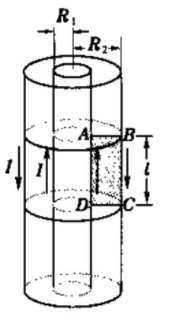
\includegraphics[scale=0.5]{2.PNG}}
 \end{figure}
  由毕奥萨伐尔定律易得,内部磁感应强度为:
 \begin{equation}
    B=\frac{\mu I}{2\pi r}
 \end{equation}
 计算流过ABCD的磁通量为
 \begin{equation}
    \varPhi=\int BdS=\int_a^bBldr=\frac{\mu_0}{2\pi}Il\int^b_a\frac{dr}{r}=\frac{\mu_0}{2\pi}Il\ln\frac{b}{a} 
 \end{equation}
 因此自感系数为:
  \begin{equation}
    L=\frac{\varPhi}{I}=\frac{\mu_0l}{2\pi}\ln\frac{b}{a} 
 \end{equation}
 我们对二者进行估算,当$\omega=2\pi f$的f大于一定的值(如f=1kHz),则有$\frac{1}{\omega C}\gg \omega L$. 考虑到同轴电缆等效电路可以等效为下图:\begin{figure}[H]\begin{center}
    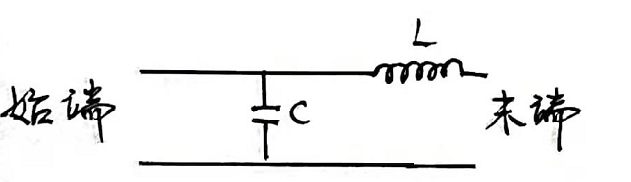
\includegraphics[scale=0.5]{11.PNG}
\end{center}\end{figure}
 因此测量电容时将传输线末端开路(电感不接入电路,无影响),测量电感时将传输线末端短路(电容的影响可以忽略).\par
 具体而言,无论是电感还是电容,我们均可以通过测量两端电压峰峰值和电流峰峰值来获得电抗值,而示波器仅能获得电压,于是我们可以通过串联一个已知电阻并测量电阻电压来获得电流值,此时我们可以计算出电抗为.\par
 \begin{equation}
    Z=\frac{V_Z}{I}=\frac{V_Z}{V_R/R}= \frac{V_Z}{V_R}\times R
    \label{qi}
 \end{equation}
 而对于电容,$Z=\frac{1}{\omega C}=\frac{1}{2\pi fC}$,故有
 \begin{equation}
    C=\frac{V_R}{V_C}\frac{1}{2\pi fR}
 \end{equation}
 测量电容时,我们将传输线末端开路,如下图,通过CH1测量电源两端电压$V_A$,通过CH2测量传输线两端电压$V_C$;通过示波器的将CH1与CH2波形相减获得电阻波形,并测量电压$V_R$,这里的电压测量均是峰峰值. 
 \begin{figure}[H]\begin{center}
    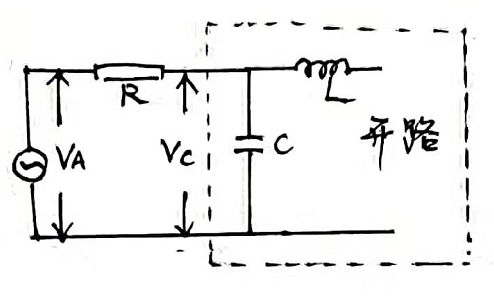
\includegraphics[scale=0.6]{12.PNG}
\end{center}\end{figure}
 为减小误差,我们在初始频率$f=60kHz$附近调整电源频率,使得$V_A$约为$V_L$($V_R$)的$\sqrt{2}$倍. 测量数据如下:

 \begin{table}[H]
    \centering
\begin{tabular}{|c|c|c|c|c|}
        \hline
        频率$f/kHz$&电阻两端$R/\Omega$&电源两端$V_A/V$&传输线两端$V_C/V$&电阻两端$V_R/V$\\
        \hline
        69.00&1000&20.384&14.651&14.697\\
        \hline
    \end{tabular}  
    \caption{电容测量数据表格} 
\end{table}
可以得到
\[C=\frac{V_R}{V_C}\frac{1}{2\pi fR}=\frac{14.697}{14.651}\times \frac{1}{2\pi\times 69.00\times 10^3\times 1000}F=2.314\times 10^{-9}F\]
传输线是由6根长度为5m同轴电缆组成的,总长$l=30m$,则单位长度的电容为:
\[C_0=\frac{C}{l}=\frac{2.314\times 10^{-9}F}{30m}=7.713\times 10^{-11}F/m\]
\subsubsection*{A.2 测量传输线等效电感}
测量等效电感的原理已于A.1部分提及,根据(\ref{qi})式,结合感抗的计算公式$Z_L=\omega L=2\pi f L$可以得到:
\begin{equation}
    L=\frac{V_LR}{2\pi fV_R}
\end{equation}
测量电容时,我们将传输线末端短路,如下图,通过CH1测量电源两端电压$V_A$,通过CH2测量传输线两端电压$V_C$;通过示波器的将CH1与CH2波形相减获得电阻波形,并测量电压$V_R$,这里的电压测量均是峰峰值. 
\begin{figure}[H]\begin{center}
    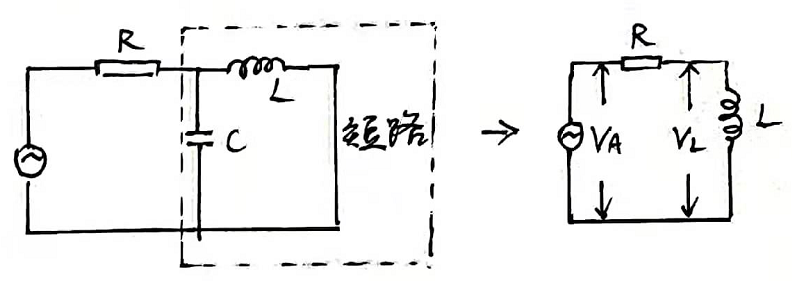
\includegraphics[scale=0.6]{13.PNG}
\end{center}\end{figure}
为减小误差,我们在初始频率$f=300kHz$附近调整电源频率,使得$V_A$约为$V_L$($V_R$)的$\sqrt{2}$倍. 测量数据如下:
\begin{table}[H]
   \centering
\begin{tabular}{|c|c|c|c|c|}
       \hline
       频率$f/kHz$&电阻两端$R/\Omega$&电源两端$V_A/V$&传输线两端$V_L/V$&电阻两端$V_R/V$\\
       \hline
       486.00&30&11.368&7.938&7.812\\
       \hline
   \end{tabular}  
   \caption{电容测量数据表格} 
\end{table}
可以得到
\[L=\frac{V_LR}{2\pi fV_R}=\frac{7.938\times 30}{2\pi\times486.00\times 10^3\times 7.812}H=9.983\times 10^{-6}H\]
传输线总长$l=30m$,则单位长度的电容为:
\[L_0=\frac{L}{l}=\frac{9.983\times 10^{-6}H}{30m}=3.328\times 10^{-7}H/m\]

\subsubsection*{A.3 趋肤效应与邻近效应}
\textbf{电力线}分布如图,其中电力线箭头方向取决于内外导体上的电荷正负,下图是其中一种情况:
\begin{figure}[H]\begin{center}
    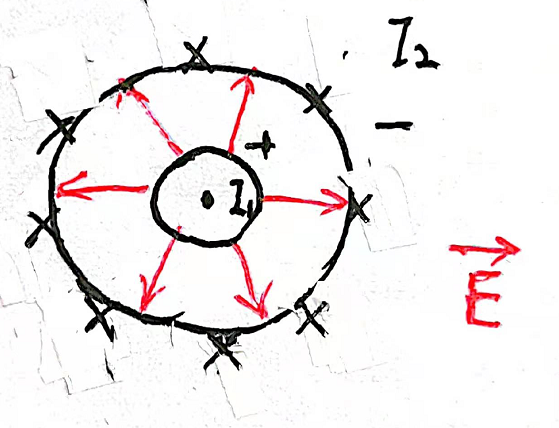
\includegraphics[scale=0.3]{14.PNG}
\end{center}\end{figure}

\textbf{磁力线}分布如图,其中外导体对内部磁场贡献为零,因此磁场由内导体产生. 磁力线箭头方向取决于内外导体上电流方向,下图是其中一种情况:
\begin{figure}[H]\begin{center}
    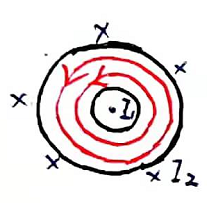
\includegraphics[scale=0.6]{15.PNG}
\end{center}\end{figure}
我们再讨论趋肤效应.\par
我们从原理上分析趋肤效应的产生原因,如下图:
\begin{figure}[H]\begin{center}
    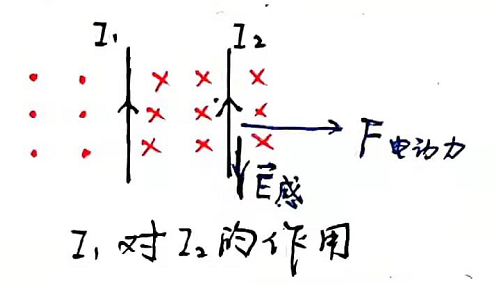
\includegraphics[scale=0.6]{16.PNG}
\end{center}\end{figure}
两条电流线同向,现在考察I1对I2的影响. 我们看到I1的磁场在I2处是指向纸面内的,如图取截面,可以看到感应电动势的方向与原来的电流相反,由此产生的感应电流向下,则根据左手定则,电动力向右,即远离电流线I1的方向;同时,I1受到I2的力也是远离的方向. 所以,在一个柱形导线中,由于电动力的存在,电流线趋于分布在柱形表面,这就是\textbf{趋肤效应}的定性解释. 同理,如果电流线方向相反,那么电动力将是靠近的方向,这就是这就是\textbf{邻近效应}的定性解释.\par
对于同轴电缆,由于对称性,外层导体电流产生的磁场在内导体处叠加为零,也即外导体不对内导体产生影响,因此由于趋肤效应,\textbf{内导体的电流主要集中在外侧}.\par
对于外导体,它类似于一个空心圆柱. 一方面,它受到自身趋肤效应的影响,将电流集中在内表面和外表面;另一方面,它还会受到内导体的电磁作用,使得电流集中在外导体内表面. 考虑到外导体与内导体的电流方向相反,那么就会产生如上所述的邻近效应. 二者会同时发生作用,但考虑到外层导体较薄,趋肤效应从两个表面向内衰减不够明显,因此邻近效应的影响更大,综上所述,\textbf{外导体电流主要集中在内侧}.


\subsection*{ B. 同轴电缆传输线的等效电路模型}
\subsubsection*{B.1 同轴电缆特征阻抗}
首先,传输线整体的\textbf{等效电路模型}为:
\begin{figure}[H]
    \centering
    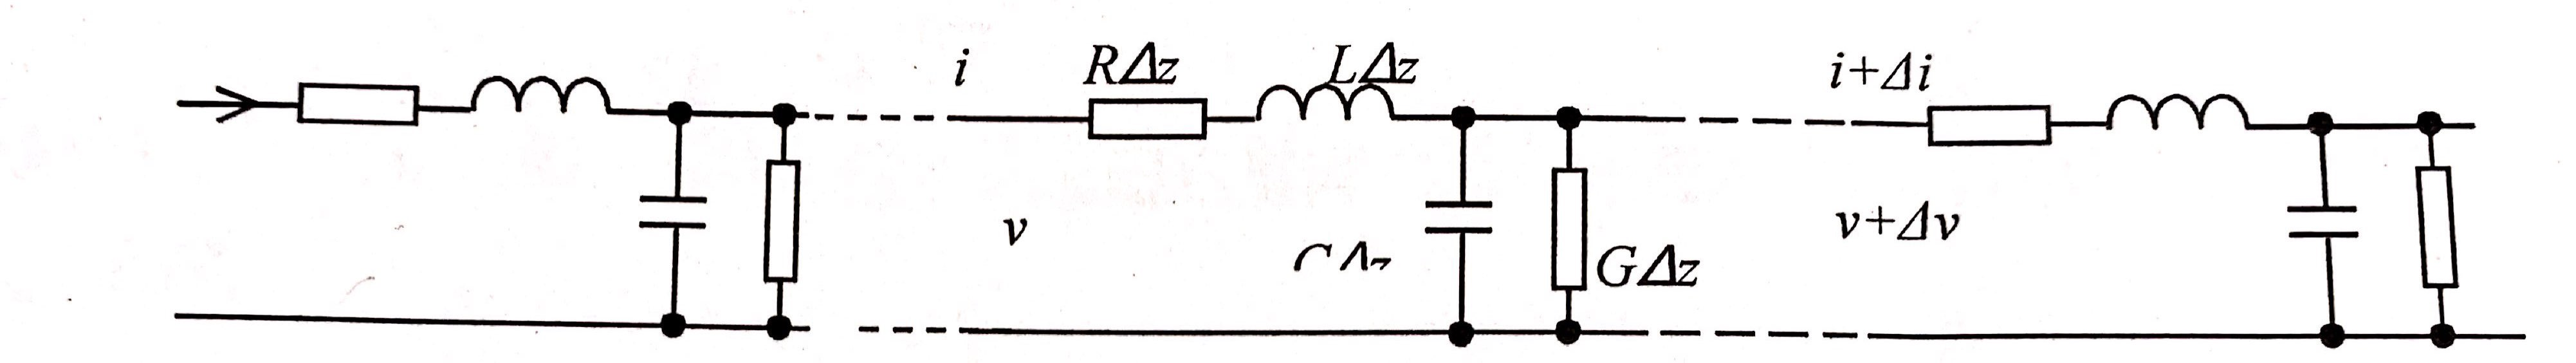
\includegraphics[width=15cm,height=2cm]{5}      
\end{figure}
其中,$R_0$、$L_0$、$C_0$、$G_0$分别为单位长度传输线的电阻、电感、电容与电导,v、i为沿
传输线方向的电压与电流,其中电压与电流均是简谐变化的,角频率为$\omega$.\par
我们取$\Delta z$长度的小段传输线,电压v经过串联阻抗产生的压降为$\Delta v=-i(R_0\Delta z+j\omega L_0\Delta z)$,电流i经过并联导纳分流为$\Delta i=-v(G_0\Delta z+j\omega C_0\Delta z)$,写作微分方程的形式则为:
\begin{equation}
   \begin{aligned}
    &\frac{\partial v}{\partial z}=-i(R_0+j\omega L_0)\\
    &\frac{\partial i}{\partial z}=-v(G_0+j\omega C_0)\\
   \end{aligned}
   \label{shi}
\end{equation}
设\textbf{传播常数$\gamma$}与\textbf{特征阻抗$Z_0$}分别为:
\begin{equation}
   \label{shiyi}
    \gamma=\sqrt{(R_0+j\omega L_0)(G_0+j\omega C_0)}=\alpha+j \beta
\end{equation}
\begin{equation}
    Z_0=\sqrt{\frac{R_0+j\omega L_0}{G_0+j\omega C_0}}
    \label{shier}
\end{equation}
则(\ref{shi})式的通解为:
\begin{equation}
   \begin{aligned}
    &v=V^+e^{-\gamma z}+V^-e^{\gamma z}\\
    &i=\frac{1}{Z_0}(V^+e^{-\gamma z}+V^-e^{\gamma z})=I^+e^{-\gamma z}+I^-e^{\gamma z}
   \end{aligned}
   \label{tongjie}
\end{equation}
那么就可得到$Z_0$的物理意义:
\begin{equation}
    Z_0=\frac{V^+}{I^+}=\frac{V^-}{-I^-}
\end{equation}

由(\ref{shier})式,当传输线无损耗时($R=G=0$),有
\begin{equation}
   \begin{aligned}
   &\gamma=j\omega\sqrt{L_0C_0}\\
   &Z_0=\sqrt{L_0/C_0}
   \end{aligned}
   \label{shiwu}
\end{equation}
故假设同轴电缆为无损耗传输线时有特征阻抗
\begin{equation}
   Z_0=\sqrt{L_0/C_0}=\sqrt{\frac{3.328\times10^{-7}H/m}{7.713\times10^{-11}F/m}}\approx65.68\Omega
\end{equation}
故无损耗传输线特征阻抗为$65.68\Omega$.

\subsubsection*{B.2 相速度和介电常数计算}

考虑到波的表示形式为$i=\frac{1}{Z_0}(V^+e^{-\gamma z}+V^-e^{\gamma z})$,这是传递过去的波及其反射波叠加得到的结果,相位的波数$k=Im(\gamma)$,而$\gamma$正是我们在(\ref{shiyi})式中得到的传播系数. 无损耗传输线的传播常数$\gamma=j\omega\sqrt{L_0C_0}$,那么该列波的波数就为$k=\omega\sqrt{L_0C_0}$,相速度可以表示为:
\begin{equation}
   v_p=\frac{\omega}{k}=1/\sqrt{L_0C_0}
   \label{shiqi}
\end{equation}
经计算得\textbf{相速度}为:
\begin{equation}
   v_p=1/\sqrt{L_0C_0}=\frac{1}{\sqrt{3.328\times10^{-7}H/m\times 7.713\times10^{-11}F/m}}\approx1.974\times 10^8m/s
\end{equation}
故相速度为$1.974\times 10^8m/s$. 而相速度在介质中表示为:
\begin{equation}
    v_p=\frac{1}{\sqrt{\mu\varepsilon}}=\frac{1}{\sqrt{\mu_r\mu_0\varepsilon_r\varepsilon_0}}
\end{equation}
在这里,我们取$\mu_r=1$,故相对介电常数为
\begin{equation}
    \varepsilon=\frac{1}{v_p^2\mu_0\varepsilon_0}
\end{equation}
考虑到$c=\frac{1}{\sqrt{\mu_0\varepsilon_0}}$,那么就有
\begin{equation}
   \varepsilon=\frac{c^2}{v_p^2}
\end{equation}
经计算得\textbf{相对介电常数}为:
\begin{equation}
   \varepsilon_r=(c/v_p)^2=(\frac{3.0\times 10^8}{1.974\times 10^8})^2=2.310
\end{equation}

故相对介电常数$\varepsilon_r= 2.310$.


\subsubsection*{B.3 信号发生器对外输出功率}
我们计算无损耗时传输线模型的电源信号输出功率. 首先我们已经计算出了忽略损耗时模型的特征阻抗为$Z_0=65.68\Omega$. 假设信号发生器电压峰峰值为$V_{PP}=10V$,频率为$f=50kHz$,并且进一步假设信号发生器电压及传输线两端实际电压,那么输出功率就为:
\[P=\frac{V_{eff}^2}{Z_0}=\frac{1}{Z_0}(\frac{V_{PP}}{2\sqrt{2}})^2=\frac{1}{65.68}(\frac{10}{2\sqrt{2}})^2W=0.190W\]
即信号发生器输出功率为0.190W. 由于没有电阻和电导,那么有功功率就为零,则输出功率全部为无功功率,这些能量全部交替存储在电容和电感中,并不断沿+z方向流动.

\subsection*{C. 脉冲信号在传输线中的传输与反射}
\subsubsection*{C.1 电压反射系数}
与B部分不同,C部分中我们需要探索的是低损耗下的同轴电缆特性. 低损耗同轴电缆传播系数和特征阻抗如下所示(证明见思考与讨论部分).
\begin{equation}
   \gamma=\alpha+j\omega\sqrt{L_0C_0}
   \label{ershisan}
\end{equation}

\begin{equation}
   Z_0\approx\sqrt{\frac{L_0}{C_0}}
   \label{ershisi}
\end{equation}
考虑一般情况,特性阻抗分别为$Z_0$和$Z_1$的传输线串联. 设幅度为$V_i$的信号通过$Z_0$到达界面,则信号会发生一定的反射. 如下图所示:
\begin{figure}[H]\begin{center}
    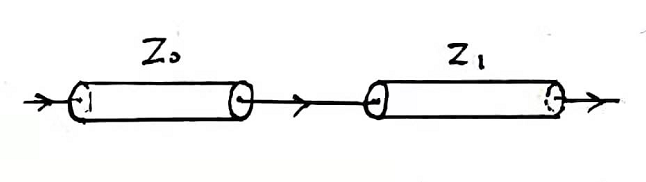
\includegraphics[scale=0.6]{17.PNG}
\end{center}\end{figure}
设透射继续传输的幅度为$V_t$,反射信号幅度为$V_r$. 根据传输线界面电压幅度相等以及电流守恒的边界条件易得:
\begin{equation}
    V_i+V_r=V_t
\end{equation}
\begin{equation}
    \frac{V_i}{Z_0}-\frac{V_r}{Z_0}=\frac{V_t}{Z_1}
\end{equation}
解得:
\begin{equation}
    V_t=\frac{2V_i}{1+\frac{Z_0}{Z_1}}
\end{equation}
\begin{equation}
    V_r=\frac{(1-\frac{Z_0}{Z_1})V_i}{1+\frac{Z_0}{Z_1}}
    \label{ershisi}
\end{equation}

定义界面处的\textbf{电压反射系数}$\Gamma=V_r/V_i$,代入得:
\begin{equation}
    \Gamma=\frac{Z_1-Z_0}{Z_1+Z_0}
    \label{ershiqi}
\end{equation}
\subsubsection*{C.2 阻抗匹配条件}

我们如果要求信号无反射,也即反射系数$\Gamma=0$,那么由(\ref{ershiqi})式得到:
\begin{equation}
    Z_0=Z_1
    \label{sanshi}
\end{equation}
此即\textbf{阻抗匹配条件},达到该条件是,信号向前传播没有反射波.
\subsubsection*{C.3 电位反向条件}
与(\ref{ershisi})式对电压幅度的推导类似,我们可以对电压进行推导,得到:
\begin{equation}
   \widetilde{U_r}=\frac{1-\frac{Z_0}{Z_1}}{1+\frac{Z_0}{Z_1}}\widetilde{U_i}
\end{equation}
因此我们可以对(\ref{ershiqi})式进行推广,将$\Gamma$的含义从电压幅值的反射系数推广到任意时刻电压值的反射系数.\par
当相位反向时,应该令$\widetilde{U_i}$前的系数,也即$\Gamma$为负数,即$\frac{Z_1-Z_0}{Z_1+Z_0}<0$,也即
\begin{equation}
   Z_1<Z_0
\end{equation}
这就是\textbf{电位反向条件},此时反射发生半波损失.

\subsubsection*{C.4 末端开路时信号传输与反射特性探究1}

由(\ref{ershiqi})式,当传输线末端为开路时,认为末端负载阻抗$Z_1=\infty$,那么利用(\ref{ershiqi})式,反射系数约为1,因此可以认为电压同相位反弹回来继续传播. 
测量传输与反射特性的电路图为:
\begin{figure}[H]
    \centering
    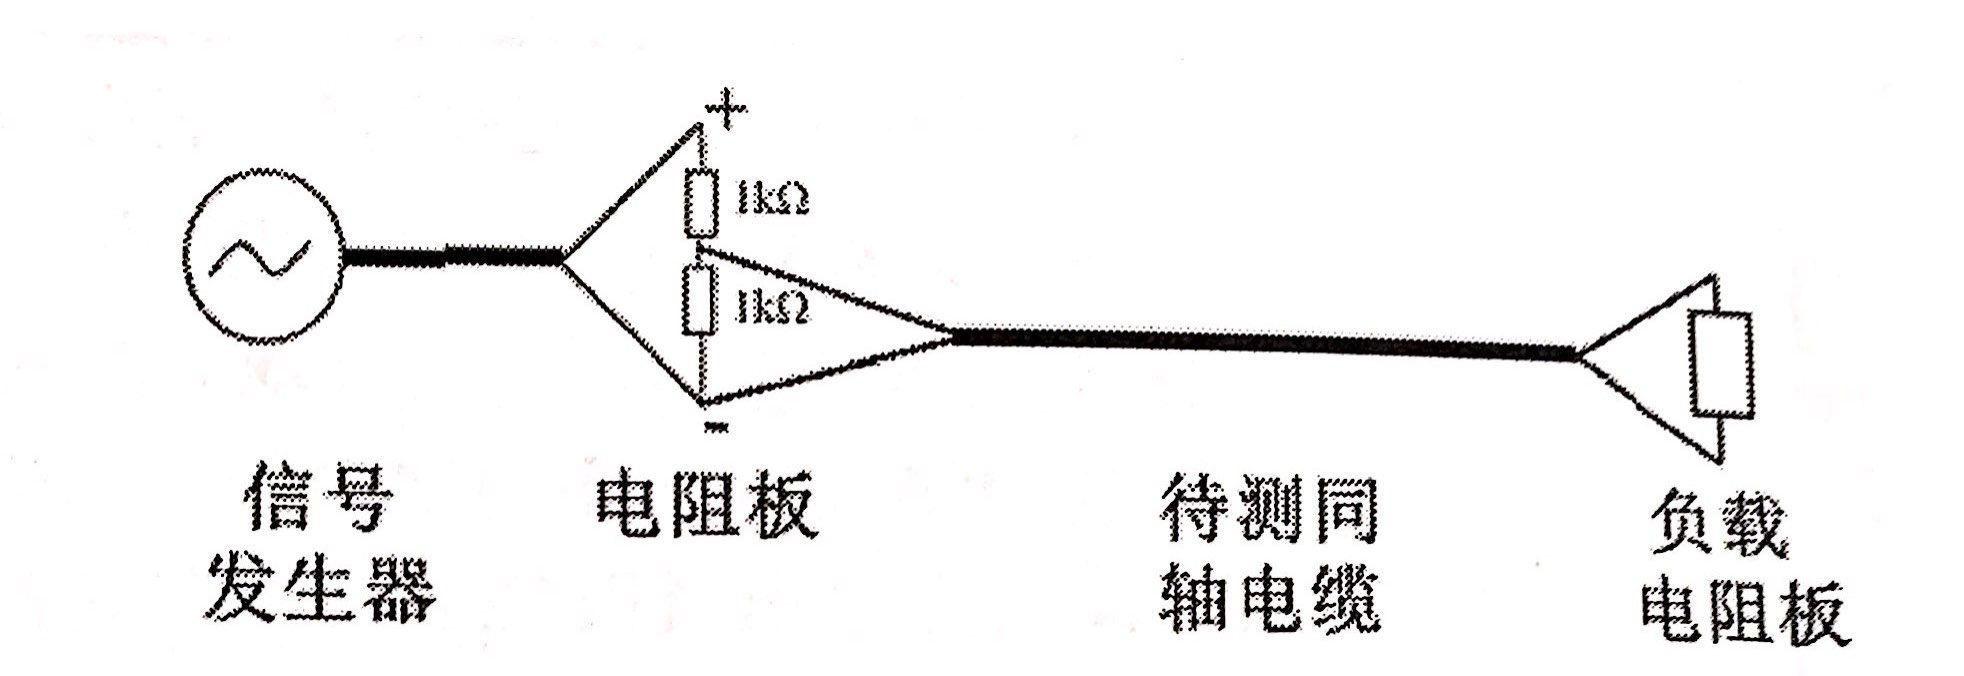
\includegraphics[width=10cm,height=3cm]{6}      
\end{figure}

其中两个$1000\Omega$电阻的作用为:由于该电阻远大于特征阻抗,也相当于开路负载,反射信号因此可被该大电阻按照同相位再次反射,从而观察到信号在电缆两端多次反射的现象. \par
我们设置信号发生器波形为脉冲,频率为40kHz,利用示波器的CH1和CH2分别测量同轴电缆起始端和末端的信号波形,记录各个波形的幅度和相对于起始脉冲的延时,测量数据见下表:
\begin{table}[H]
   \centering
\begin{tabular}{|c|c|c|}
       \hline
       &信号幅度$V_i/V$&信号延迟$\tau_i/ns$\\
       \hline
       $V_0$与$\tau_0$&$1.28$&0\\
       \hline
       $V_1$与$\tau_1$&$2.10$&134\\ 
       \hline
       $V_2$与$\tau_2$&$1.83$&278\\ 
       \hline
       $V_3$与$\tau_3$&$1.34$&424\\ 
       \hline
       $V_4$与$\tau_4$&$1.17$&570\\ 
       \hline
       $V_5$与$\tau_5$&$0.88$&718\\ 
       \hline
       $V_6$与$\tau_6$&$0.77$&864\\ 
       \hline
   \end{tabular}  
   \caption{末端开路时始端与末端信号幅度及延迟数据表} 
\end{table} 
其中,各$V_i$的含义见下图:
\begin{figure}[H]
    \centering
    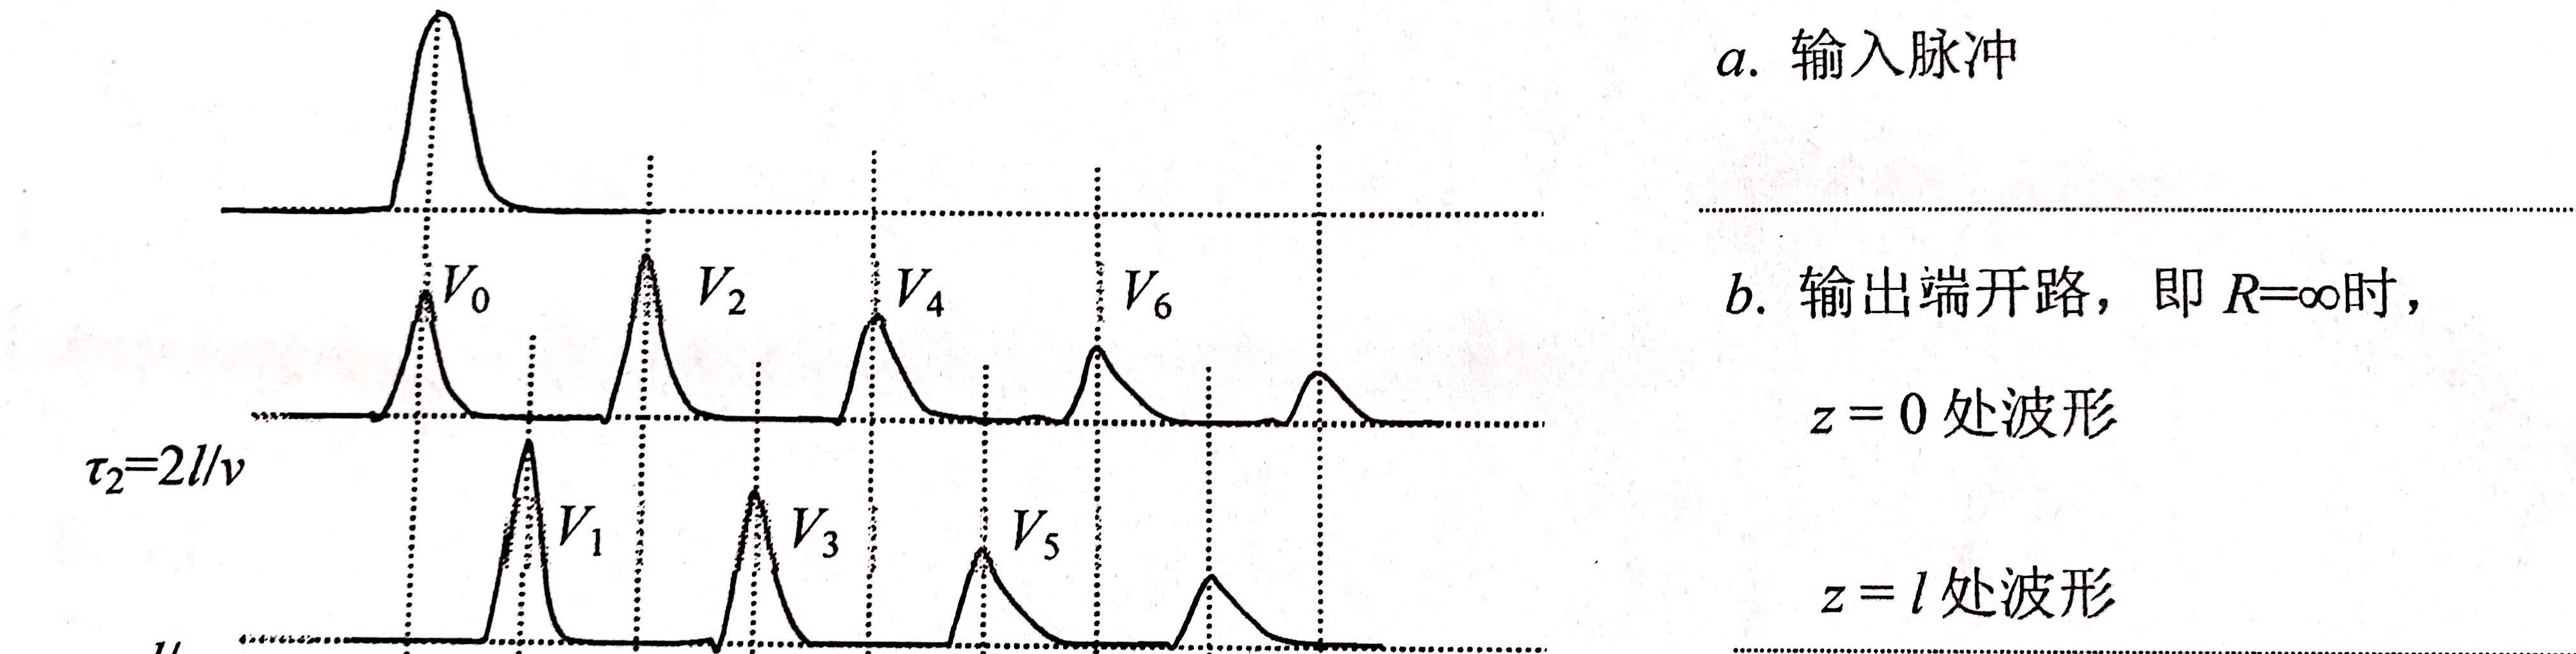
\includegraphics[width=15cm,height=3cm]{7}      
\end{figure}
其中$V_0$是初始$z=0$处测得的进入同轴电缆的信号,之后信号经过反射再次回到$z=0$处,$V_2$就是入射和反射信号叠加后的波形;信号再经$z=0$处反射后形成$V_4$,以此类推. $V_1, V_3...$是在$z=l$处反射1次、2次......后形成的入射和反射信号叠加波形.\par
实际测量结果见下图:
\begin{figure}[H]\begin{center}
    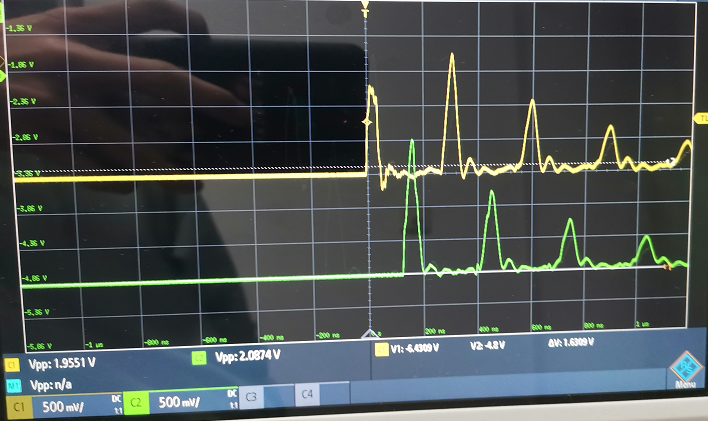
\includegraphics[scale=0.7]{31.PNG}
\end{center}\end{figure}
这里我们测量始端信号和末端信号时入射和反射信号被叠加在了一起.

\subsubsection*{C.4 末端开路时信号传输与反射特性探究2}
考虑到C.3中始端信号和末端信号时入射和反射信号被叠加,无法区别出入射和反射信号,因此我们在$z=5/6l$处测量波形,这样入射波与反射波在时间轴上被分开了,这样更便于我们观察。具体情况见下图:
\begin{figure}[H]\begin{center}
    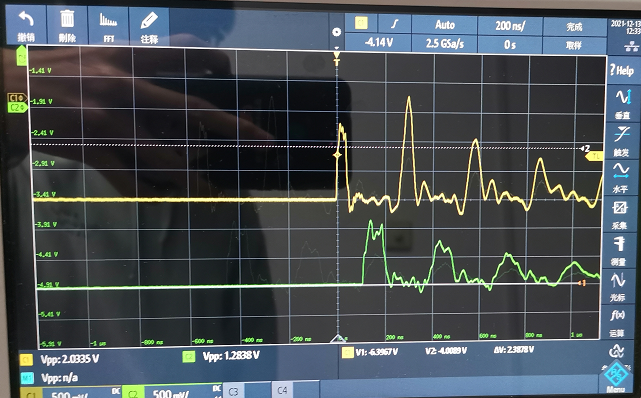
\includegraphics[scale=0.7]{32.PNG}
\end{center}\end{figure}
其中,$Z=5/6l$图像前两个峰(记为1'与2')分别为入射和反射波形. 其幅度分别为$V_1'=1.14V$,$V_2'=1.07V$,则二者的叠加(求和)为:
\begin{equation}
    V_{sum}=V_1'+V_2'=1.14+1.07V=2.21V
\end{equation}
而 表3 中给出的$V_1=2.10V$,$V_1$与$V_{sum}$存在误差,但基本相等,二者吻合得较好,验证了实验原理和操作的正确性.

\subsubsection*{C.6 末端短路时传输与反射特征}
末端短路时,相当于$Z_l=0<Z_0$,此时信号在末端反射且相位相反反向,沿-z方向传输.\par
实际实验时,我们利用导线将传输线末端短路,同时始端仍然保持高电阻以达到反射的目的. 利用示波器观察起始端(末端短路,故末端信号幅度为0,无需观察)信号幅度和相对起始脉冲延时数据为:
\begin{table}[H]
    \centering
\begin{tabular}{|c|c|c|}
        \hline
        &信号幅度$V_i/V$&信号延迟$\tau_i/ns$\\
        \hline
        $V_0$与$\tau_0$&$1.33$&0\\
        \hline
        $V_2$与$\tau_2$&$-1.88$&300\\ 
        \hline
        $V_4$与$\tau_4$&$1.55$&598\\ 
        \hline
        $V_6$与$\tau_6$&$-0.756$&896\\ 
        \hline
    \end{tabular}  
    \caption{末端短路时始端信号幅度及延迟数据表} 
\end{table} 

其中,各$V_i$的含义见下图:
\begin{figure}[H]
    \centering
    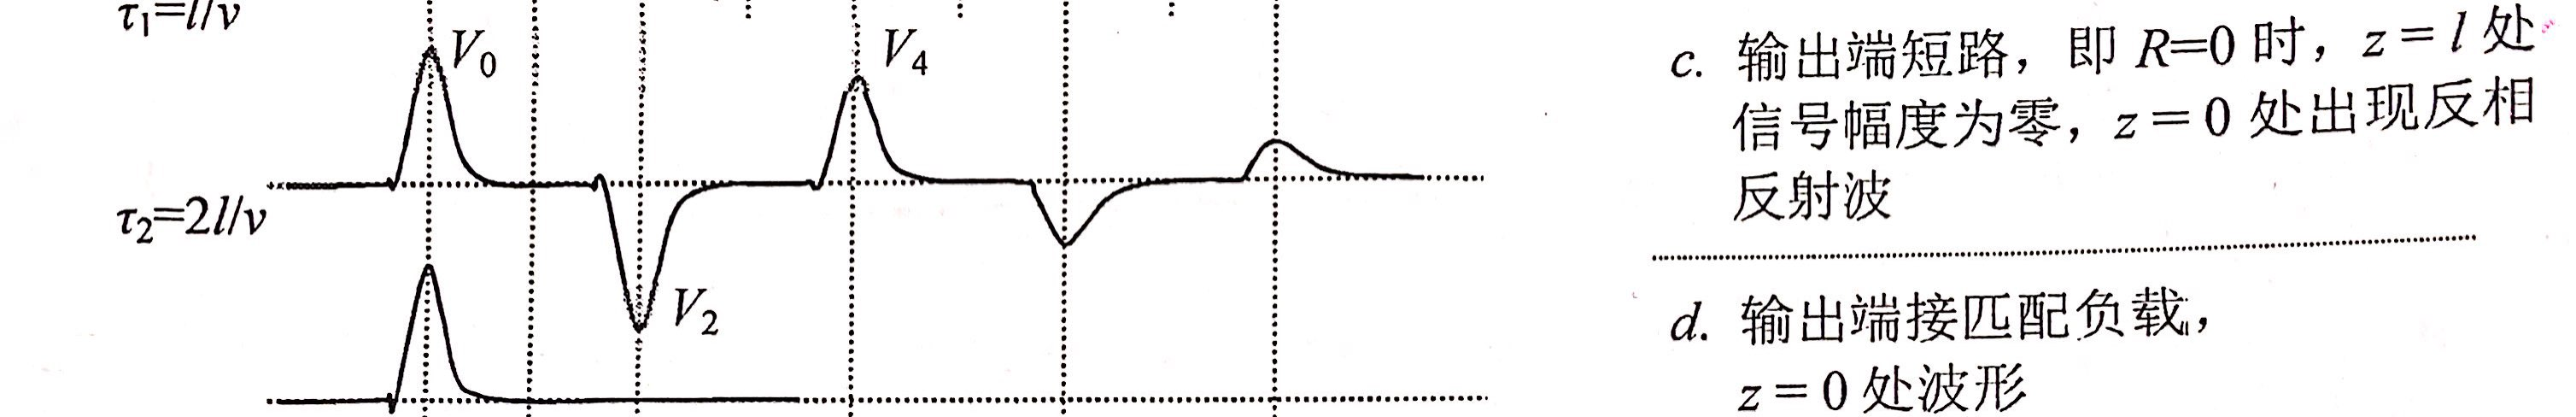
\includegraphics[width=15cm,height=3cm]{9}      
\end{figure}
实际观测到的波形如下:

\begin{figure}[H]\begin{center}
    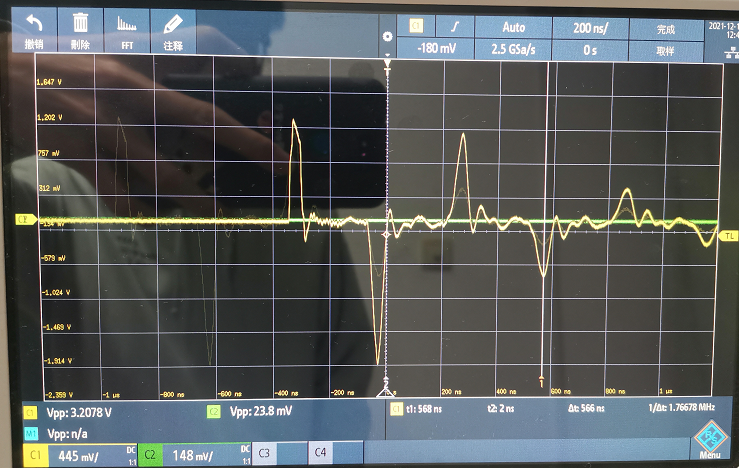
\includegraphics[scale=0.7]{33.PNG}
\end{center}\end{figure}
我们同样引入$z=5/6l$处的波形图,分开观察入射波与反射波:

\begin{figure}[H]\begin{center}
    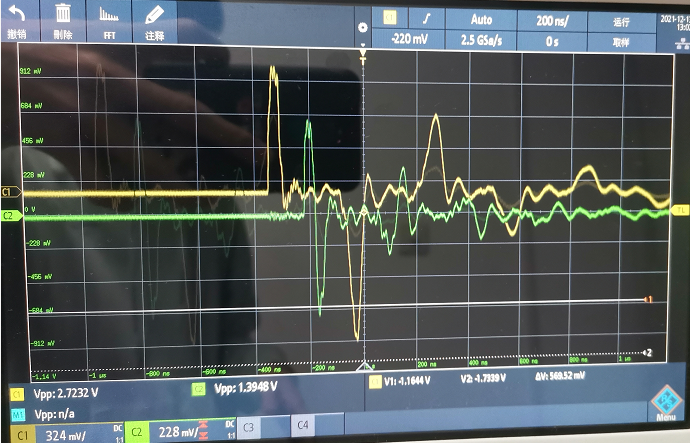
\includegraphics[scale=0.7]{34.PNG}
\end{center}\end{figure}

其中,$Z=5/6l$图像前两个峰(记为1'与2')分别为入射和反射波形,
其幅度分别为$V_1'=1.49V$,$V_2'=-1.43V$,则二者的叠加(求和)为:
\begin{equation}
    V_{sum}=V_1'+V_2'=1.49-1.43V=0.06V
\end{equation}

而理论上末端短路,两个峰的叠加幅度应为0。二者存在误差,但相对于$V_1'$与$V_2'$的数值
而言该误差较小,因此可以认为仍在误差范围内近似相等.

\subsubsection*{C.7 末端接负载时测量传输线特征阻抗}
\textbf{末端接负载}时,即$Z_l=R$。由(\ref{sanshi})给出的结论,当$Z_l=Z_0$时,此时信号被负载吸收,达到阻抗匹配条件;此时信号完全透射而没有反射,
即只有沿+z方向传播的行波.\par

在实验中,我们使用以$10\Omega$为单位的串联电阻板作为负载接入传输线末端,改变负载阻值使得反射波幅度达到最小,则理论上,此时的阻值与传输线特性阻抗相同.\par
实际测量时,我们将示波器CH1接入传输线$z=5/6l$处,并观察第二个波峰,该波峰为反射信号. 测量数据如下:
\begin{table}[H]
    \centering
\begin{tabular}{|c|c|}
        \hline
        负载电阻$R/\Omega$&反射信号波峰峰值$V_i/V$\\
        \hline
        40&1.60\\
        \hline
        50&1.52\\ 
        \hline
        60&1.51\\ 
        \hline
        70&1.58\\ 
        \hline
        80&1.61\\ 
        \hline
    \end{tabular}  
    \caption{末端接负载时反射信号数据表} 
\end{table} 
我们可以看到反射信号最小时$R=60\Omega$. 由于负载阻值只能以$10\Omega$为单位变化,故该数据与 B.1 计算所得的特征阻抗$65.68\Omega$基本相符,再次验证了实验原理和操作的正确性.

\subsubsection*{C.8 计算同轴电缆衰减系数}
由(\ref{ershisan})式,衰减系数为$\gamma=\alpha+j\omega\sqrt{L_0C_0}$,代入(\ref{tongjie})式得低损耗同轴电缆传输时信号
\begin{equation}
v=V^+e^{-\gamma z}+V^-e^{\gamma z}=V^+e^{(-\alpha-j\omega\sqrt{L_0C_0})z}+V^-e^{(\alpha+j\omega\sqrt{L_0C_0})z}
\end{equation}
此式前一项是+z方向传播的信号,后一项是-z方向反射的信号. 我们只研究+z方向的信号,则有
\begin{equation}
    v=V_0e^{(-\alpha-j\omega\sqrt{L_0C_0})z}=V_0e^{-\alpha z}e^{-j\omega\sqrt{L_0C_0}z}
    \label{sanshiliu}
\end{equation}
则$e^{-j\omega\sqrt{L_0C_0}z}$项是在描述沿+z方向的振动,而$e^{-\alpha}z$描述的是该振动的衰减情况,故可以定义$\alpha$为衰减系数,幅度为$V_0$的信号经过长为l的电缆后信号幅度为$V=V_0e^{-\alpha l}$,故有:
\begin{equation}
    \ln{V}=-\alpha l+\ln{V_0}
    \label{sanshiqi}
\end{equation}
于是我们可以通过直线拟合$l$与$\ln{V}$的关系来计算衰减系数. 而$l$与$\ln{V}$的数据可以由C.4获得. 各个信号的幅度之含义已经在C.4介绍过,鉴于除了$V_0$之外的所有数据测量值均为入射与反射叠加,我们不妨取$V_1-V_6$一半为实际幅度. 我们计算出的数据如下表所示:
\begin{table}[H]
    \centering
\begin{tabular}{|c|c|c|c|}
        \hline
        序号&$V_i/V$&$\ln{V_i}/\ln{V}$&l/m\\
        \hline
        1&1.28&0.247&0\\ 
        \hline
        2&1.05&0.049&30\\ 
        \hline
        3&0.92&-0.089&60\\ 
        \hline
        4&0.67&-0.400&90\\ 
        \hline
        5&0.59&-0.536&120\\ 
        \hline
        6&0.44&-0.821&150\\ 
        \hline
        7&0.39&-0.955&180\\ 
        \hline
    \end{tabular}  
    \caption{$l$与$\ln{V}$的数据表格}
\end{table} 
利用OriginPro进行直线拟合,得到的曲线如下:
\begin{figure}[H]
    \centering{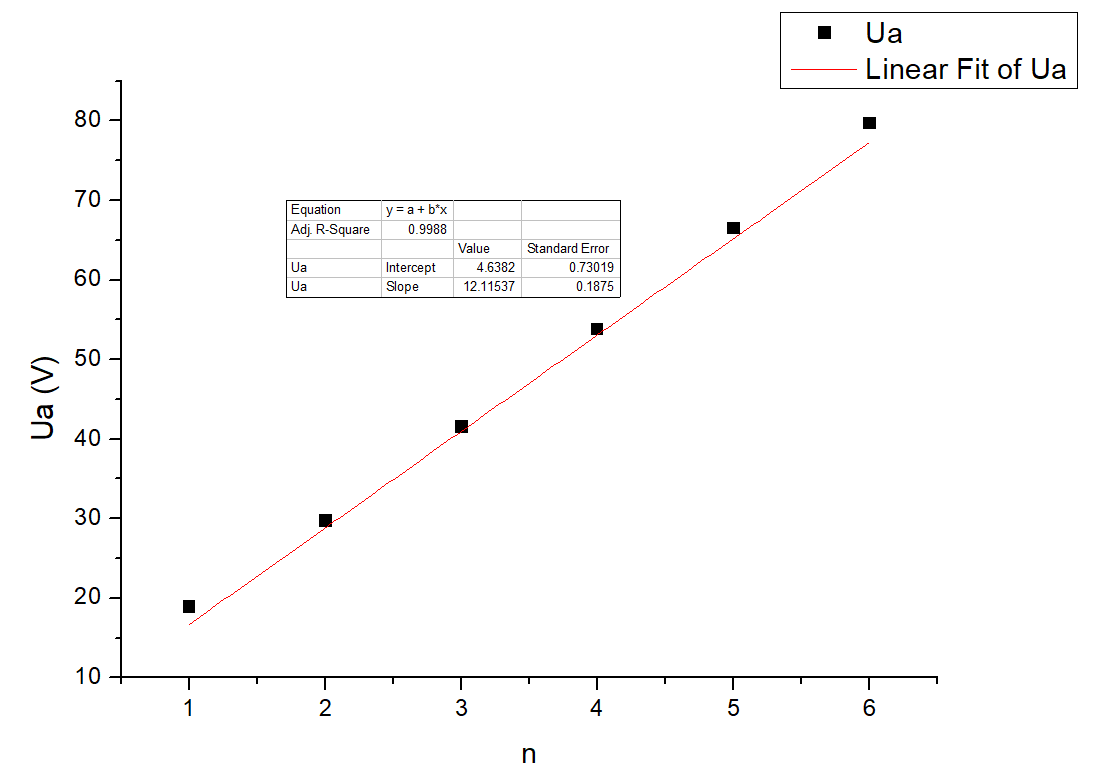
\includegraphics[scale=0.5]{linear.PNG}}
\end{figure}
该直线拟合$R^2=0.99187$,考虑到众多误差因素,拟合情况还是较好的. 从结果中我们获知拟合直线斜率为$k=-0.00689m^{-1}$,故有衰减系数
\[\alpha\approx 0.00689m^{-1}\]
\subsubsection*{C.9 信号衰减}
(1)$V_0$幅度小于$V_1$:我们在C.4部分中已经叙述过各个波形对应的信号. $V_0$为单个的入射信号幅度,而$V_1$为入射与反射叠加的信号幅度,大致为单个幅度的两倍. 虽然信号从$V_0$到$V_1$在传输线中有所衰减,但衰减较为缓慢,故
$V_1$仍大于$V_0$.

(2)从$V_1$后信号幅度逐步衰减:由 C.8 知信号有衰减系数,(\ref{sanshiliu})和(\ref{sanshiqi})式均描述了信号强度随着传播距离的增大而指数级下降的现象. 考虑到$V_1-V_6$均是入射信号和反射信号叠加获得的,且传播距离依次增加,则信号幅度逐步衰减也是自然的现象.

\subsection*{D. 简谐信号在传输线中的驻波}
\subsubsection*{D.1 末端开路形成驻波理论推导}
我们将信号发生器仍调回正弦波,并由(\ref{tongjie})式可以得到
\[v=V^+e^{-\gamma z}+V^-e^{\gamma z}\]
此式前一项是+z方向传播的信号,后一项是-z方向反射的信号. 我们将它们分离开;信号传播要考虑时间,故还需乘以时间系数$e^{j\omega t}$(其中$\omega$即为相速度$v_p$的角速度)设$V^+(z)$为沿传输线+z方向的入射电压信号,$V^-(z)$为沿-z方向的反射信号,则二者表达式为:
\begin{equation}
    \begin{aligned}
    &V^+(z)=V^+ e^{j\omega t-\gamma z+j\varphi^+}\\
    &V^-(z)=V^- e^{j\omega t+\gamma z+j\varphi^-}
    \end{aligned}\label{sanshijiu}
\end{equation}
我们先考虑末端开路的情况. 由于初、末端均为开路,故信号反射前后无相位差和幅值改变,故有$V^+(l)=V^-(l)$(详见C.4),而形成驻波的条件是$z=0$处从末端反射回的信号和初始的信号保持一致,故有$V^+(0)=V^-(0)$,则幅值变化和初、末端边界条件可以总结为:
\begin{equation}
    \begin{aligned}
    &V^+=V^-\\
    &V^+(0)=V^-(0)\\
    &V^+(l)=V^-(l)
    \end{aligned}
\end{equation}
代入(\ref{sanshijiu})式,可以推导出:
\begin{equation}
    \begin{aligned}
        &\varphi^+=\varphi^-+2n\pi\\
        &\varphi^+=2\gamma l/j+\varphi^-+2n'\pi
    \end{aligned}
\end{equation}
故有\begin{equation}\gamma l=n\pi j(n\in \mathbb{Z}_+)\label{sishier}\end{equation}\\
我们将传输线简化为无损耗的同轴电缆,则由(\ref{shiwu})式有,$\gamma=j\omega\sqrt{L_0C_0}=2j\pi f\sqrt{L_0C_0}$,由(\ref{shiqi})式有$v_p=1/\sqrt{L_0C_0}$,代入上式得
\begin{equation}f=\frac{n}{2l\sqrt{L_0C_0}}=\frac{nv_p}{2l}(n\in \mathbb{Z}_+)\label{sishier}
\end{equation}
这就是形成驻波时信号频率$f$应符合的条件.


\subsubsection*{D.2 末端开路形成驻波计算}
结合$l=30m$以及$v_p=1.974\times 10^8m/s$并令$n=1$与$n=2$,代入(\ref{sishier})式得最小的两个频率为:
\begin{equation}
    f_1=\frac{v_p}{2l}=\frac{1.974\times 10^8m/s}{2\times 30m}=3.290MHz
\end{equation}
\begin{equation}
    f_2=\frac{v_p}{l}=\frac{1.974\times 10^8m/s}{30m}=6.580MHz
\end{equation}
即形成驻波最低的两个频率为$f_1=3.290MHz$和$f_2=6.580MHz$.


\subsubsection*{D.3 观察末端开路形成的驻波}
得到(\ref{sishier})式后,我们将(\ref{sanshijiu})式相加获得叠加信号:
\begin{equation}
    \begin{aligned}
        v&=V^+(z)+V^-(z)\\ 
        &=V^+e^{j\omega t-\gamma z+j\varphi^+}+V^- e^{j\omega t+\gamma z+j\varphi^-}\\
        &=V^+e^{j\omega t-\frac{n\pi}{l}j z+j\varphi^+}+V^+ e^{j\omega t+\frac{n\pi}{l}j z+j(\varphi^++2\pi)}\\
        &=V^+(\cos(\omega t-\frac{n\pi}{l}z+\varphi^+)+\cos(\omega t+\frac{n\pi}{l}z+\varphi^+))\\
        &=2V^+\cos(\omega t+\varphi^+)\cos(\frac{n\pi}{l}z)
    \end{aligned}
    \label{zhubo}
\end{equation}
此式前一项是驻波随时间变化的情况,后一项是空间分布因子. 信号发生器已置于正弦波波形,我们激昂电压峰峰值调至10$V_{PP}$,并将示波器CH1接入传输线始端,CH2接入$z=1/2l$处,CH3接入传输线终端,并将信号发生器频率分别调至$f_1=3.290MHz$和$f_2=6.580MHz$分$n=1$和$n=2$两种情况观察波形.\par


(1)$n=1$时:\\

依据(\ref{zhubo}),将之改写为:
\begin{equation}
    v=2V^+\cos(\omega t+\varphi^+)\cos(\frac{\pi}{l}z)
    \label{n=1}
\end{equation}\par
理论上始端($\cos{0}=1$)与末端($\cos{\pi}=-1$)应该振幅最大、相位相反;中间处($\cos{\frac{1}{2}\pi}=0$)振幅应当为0. \\
实际波形图如下:

\begin{figure}[H]\begin{center}
    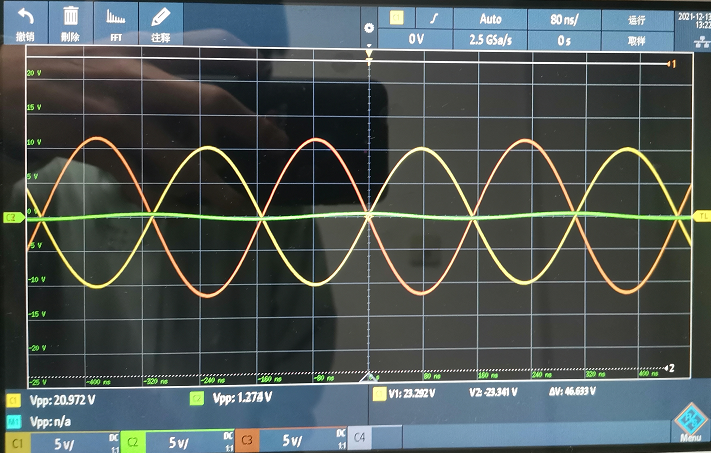
\includegraphics[scale=0.7]{21.PNG}
\end{center}\end{figure}

(2)$n=2$时:\\

依据(\ref{zhubo}),将之改写为:
\begin{equation}
    v=2V^+\cos(\omega t+\varphi^+)\cos(\frac{2\pi}{l}z)
    \label{n=2}
\end{equation}\par
理论上始端($\cos{0}=1$)与末端($\cos{2\pi}=1$)振幅最大、相位相同;中间处($\cos{\pi}=-1$)振幅也最大,但相位相反.\\
实际波形图如下:

\begin{figure}[H]\begin{center}
    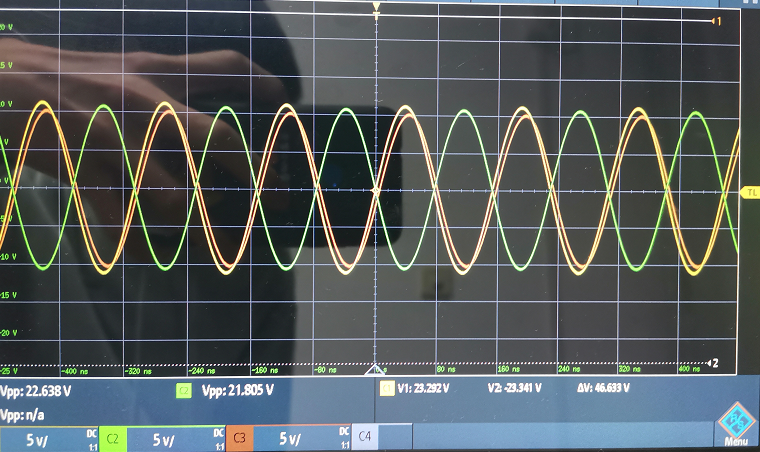
\includegraphics[scale=0.7]{22.PNG}
\end{center}\end{figure}


\subsubsection*{D.4 末端开路时电压信号幅度分布示意图}
由(\ref{n=1})和(\ref{n=2})式得,$n=1$和$n=2$空间分布因子分别为$\cos(\frac{\pi}{l}z)$和$\cos(\frac{2\pi}{l}z)$,将二者画在一张图中,则如下图所示(考虑到横坐标是振幅,故需要对空间分布因子取绝对值):

\begin{figure}[H]\begin{center}
    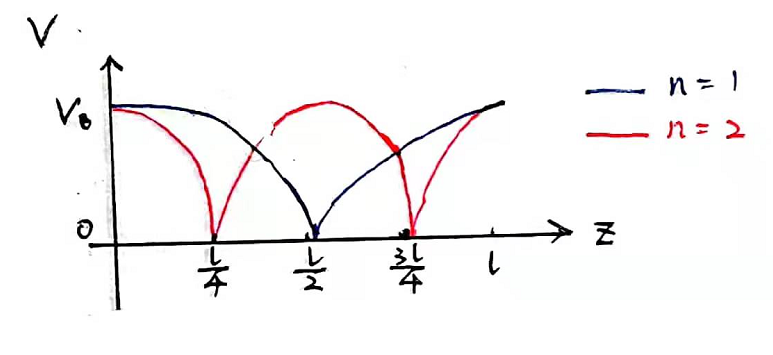
\includegraphics[scale=0.6]{18.PNG}
\end{center}\end{figure}


\subsubsection*{D.5 末端短路时的驻波}
仿照D.1中的推导,我们进行末端短路时的推导. 我们观察(\ref{sanshijiu})式,并寻找边界条件约束. 由于末端为短路,故信号反射前后相位相差$\pi$,但幅值绝对值不变,故有$V^+(l)=V^-(l)e^{j\pi}$(也可以写作$V^+(l)=-V^-(l)$,详见C.6),而形成驻波的条件是$z=0$处从末端反射回的信号和初始的信号保持一致,故有$V^+(0)=V^-(0)$,则幅值变化和初、末端边界条件可以总结为:
\begin{equation}
    \begin{aligned}
    &V^+=V^-\\
    &V^+(0)=V^-(0)\\
    &V^+(l)=-V^-(l)
    \end{aligned}
\end{equation}
代入(\ref{sanshijiu})式,可以推导出:
\begin{equation}
    \begin{aligned}
        &\varphi^+=\varphi^-+2n\pi\\
        &\varphi^+=2\gamma l/j+\varphi^-+(2n'+1)\pi
    \end{aligned}
\end{equation}
故有\begin{equation}\gamma l=\frac{2n-1}{2}\pi j(n\in \mathbb{Z}_+)\label{sishier2}\end{equation}\\

我们将传输线简化为无损耗的同轴电缆,则由(\ref{shiwu})式有,$\gamma=j\omega\sqrt{L_0C_0}=2j\pi f\sqrt{L_0C_0}$,由(\ref{shiqi})式有$v_p=1/\sqrt{L_0C_0}$,代入上式得
\begin{equation}f=\frac{2n-1}{4l\sqrt{L_0C_0}}=\frac{(2n-1)v_p}{4l}(n\in \mathbb{Z}_+)\label{sishier2}
\end{equation}
这就是形成驻波时信号频率$f$应符合的条件.
结合$l=30m$以及$v_p=1.974\times 10^8m/s$并令$n=1$与$n=2$,代入(\ref{sishier})式得最小的两个频率为:
\begin{equation}
    f_1=\frac{v_p}{4l}=\frac{1.974\times 10^8m/s}{4\times 30m}=1.645MHz
\end{equation}
\begin{equation}
    f_2=\frac{3v_p}{4l}=\frac{3\times 1.974\times 10^8m/s}{4\times 30m}=4.935MHz
\end{equation}
即形成驻波最低的两个频率为$f_1=1.645MHz$和$f_2=4.935MHz$.
得到(\ref{sishier2})式后,我们将(\ref{sanshijiu})式相加获得叠加信号:
\begin{equation}
    \begin{aligned}
        v&=V^+(z)+V^-(z)\\ 
        &=V^+e^{j\omega t-\gamma z+j\varphi^+}+V^- e^{j\omega t+\gamma z+j\varphi^-}\\
        &=V^+e^{j\omega t-\frac{2n-1}{2}j z+j\varphi^+}+V^+ e^{j\omega t+\frac{2n-1}{2}{l}j z+j(\varphi^++2\pi)}\\
        &=V^+(\cos(\omega t-\frac{2n-1}{2}z+\varphi^+)+\cos(\omega t+\frac{2n-1}{2}z+\varphi^+))\\
        &=2V^+\cos(\omega t+\varphi^+)\cos(\frac{2n-1}{2}z)
    \end{aligned}
    \label{zhubo2}
\end{equation}
此式前一项是驻波随时间变化的情况,后一项是空间分布因子. 信号发生器已置于正弦波波形,我们激昂电压峰峰值调至10$V_{PP}$,并将示波器CH1接入传输线始端,CH2接入$z=1/2l$处,CH3接入传输线终端,并将信号发生器频率分别调至$f_1=1.645MHz$和$f_2=4.935MHz$分$n=1$和$n=2$两种情况观察波形.\par

(1)$n=1$时:\\

依据(\ref{zhubo2}),将之改写为:
\begin{equation}
    v=2V^+\cos(\omega t+\varphi^+)\cos(\frac{\pi}{2l}z)
    \label{n=1'}
\end{equation}\par
理论上始端($\cos{0}=1$)振幅最大;末端($\cos{\frac{1}{2}\pi}=0$)没有振幅;中间处($\cos{\frac{1}{4}\pi}=\frac{\sqrt{2}}{2}$)振幅应该位于二者之间.\\
实际波形图如下:

\begin{figure}[H]\begin{center}
    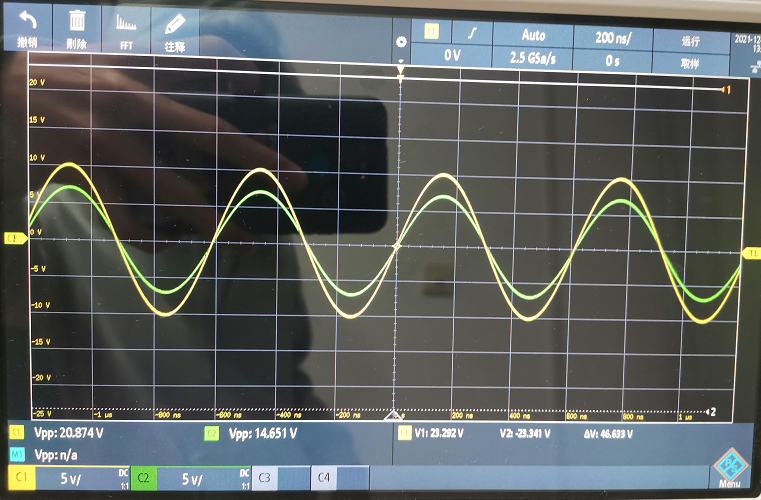
\includegraphics[scale=0.7]{23.PNG}
\end{center}\end{figure}

(2)$n=2$时:\\

依据(\ref{zhubo2}),将之改写为:
\begin{equation}
    v=2V^+\cos(\omega t+\varphi^+)\cos(\frac{3\pi}{2l}z)
    \label{n=2'}
\end{equation}\par
理论上始端($\cos{0}=-1$)振幅最大,末端($\cos{\frac{3}{2}\pi}=0$)没有振幅;中间处($\cos{\frac{3}{4}\pi}=-\frac{\sqrt{2}}{2}$)振幅居中.\\
实际波形图如下:

\begin{figure}[H]\begin{center}
    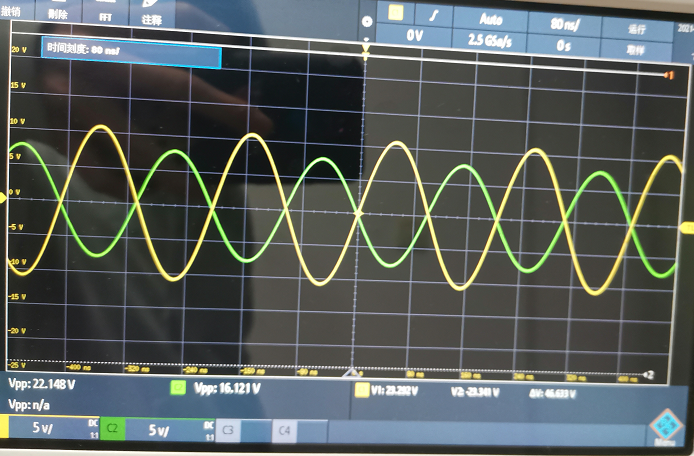
\includegraphics[scale=0.7]{24.PNG}
\end{center}\end{figure}

由(\ref{n=1})和(\ref{n=2})式得,$n=1$和$n=2$空间分布因子分别为$\cos(\frac{\pi}{2l}z)$和$\cos(\frac{3\pi}{2l}z)$,将二者画在一张图中,则如下图所示(考虑到横坐标是振幅,故需要对空间分布因子取绝对值):

\begin{figure}[H]\begin{center}
    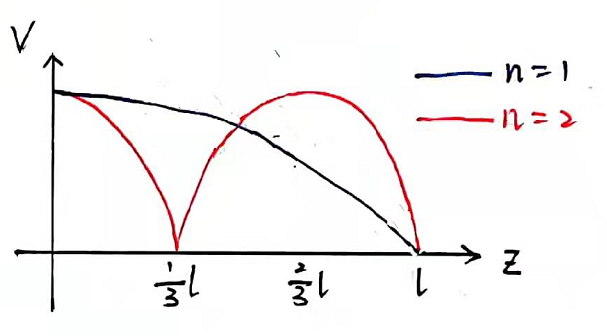
\includegraphics[scale=0.6]{19.PNG}
\end{center}\end{figure}







\section{思考与讨论}
\subsection*{1. 同轴电缆低损耗情况下传播系数(\ref{ershisan})式和特征阻抗(\ref{ershisi})式的推导}
我们要通过对(\ref{shiyi})式和(\ref{shier})式作进一步分析得到推导,\par
当传输线很小时,也即$R\ll \omega L$和$G\ll \omega C$时,将(\ref{shiyi})式展开到一阶小量,有
\begin{equation}
    \begin{aligned}
      \gamma&=\sqrt{(R_0+j\omega L_0)(G_0+j\omega C_0)}\\
      &=(1+\frac{R_0}{2j\omega L_0})(1+\frac{G_0}{2j\omega C_0})j\omega\sqrt{L_0C_0}\\
      &=(\frac{R_0}{2L}+\frac{G_0}{2C_0})\sqrt{L_0C_0}+(1-\frac{R_0G_0}{4\omega^2C_0L_0})j\omega\sqrt{L_0C_0}
    \end{aligned}
\end{equation}
实部仅有一阶无穷小,考虑到实部表示衰减系数,则保留实部的一阶无穷小;虚部忽略一阶无穷小,则有:
\begin{equation}
   \gamma=\alpha+j\omega\sqrt{L_0C_0}
\end{equation}
其中\begin{equation}\alpha\approx(\frac{R_0}{2L_0}+\frac{G_0}{2C_0})\sqrt{L_0C_0}\label{alpha}\end{equation}
将(\ref{shier})式展开到一阶小量,有
\begin{equation}
   \begin{aligned}
      Z_0&=\sqrt{\frac{R_0+j\omega L_0}{G_0+j\omega C_0}}\\
         &=\sqrt{\frac{R_0/j\omega L_0+1}{G_0/j\omega C_0+1}}\sqrt{\frac{L_0}{C_0}}\\
         &=(1+\frac{R_0}{2j\omega L_0})(1-\frac{G_0}{2j\omega C_0})\sqrt{\frac{L_0}{C_0}}\\
         &=(1+\frac{R_0G_0}{4\omega^2C_0L_0}+\frac{R_0}{2j\omega L_0}-\frac{G_0}{2j\omega C_0})\sqrt{\frac{L_0}{C_0}}\\
   \end{aligned}
\end{equation}
在这里,我们忽略实部的一阶小量,同时考虑到虚部均为一阶小量,于是也将虚部忽略($Z_0$的虚部并没有$\gamma$的实部一般具有实际意义,因此可以将$Z_0$的虚部整个忽略),可以得到:
\begin{equation}
    Z_0\approx\sqrt{\frac{L_0}{C_0}}
\end{equation}
以上就是传输线低损耗时的传播系数和特征阻抗.\par

\subsection*{2. 衰减系数$\alpha$的估算}
事实上,我们已经通过(\ref{alpha})式得知在低损耗下的同轴电缆衰减系数大约为\begin{equation}\alpha\approx(\frac{R_0}{2L_0}+\frac{G_0}{2C_0})\sqrt{L_0C_0}=\frac{R_0}{2Z_0}+\frac{Z_0G_0}{2}\label{a}\end{equation},我们将利用此式对同轴电缆衰减常数做估算.

同轴电缆的单位电阻和电导推导如下\footnote{详见:波扎尔 D.M., 张肇仪, 周乐柱等. 微波工程[M]. 北京: 电子工业出版社, 2015:46-47.}:
\begin{equation}
    R=\frac{R_s}{(2\pi)^2}(\int_{\phi=0}^{2\pi}\frac{1}{a^2}ad\phi+\int_{\phi=0}^{2\pi}\frac{1}{b^2}bd\phi)=\frac{R_s}{2\pi}(\frac{1}{a}+\frac{1}{b})
\end{equation}
\begin{equation}
    G=\frac{\omega \varepsilon'}{(\ln b/a)^2\int^{2\pi}_{\phi=0}\int^{b}_{\rho =a}\frac{1}{\rho^2}\rho d\rho d\phi}=\frac{2\pi \varepsilon'\omega}{\ln b/a}
\end{equation}
计算得下列物理量数量级:$R_0\approx 10\Omega/m$,$G_0\approx 10^{-6}S/m$,而我们前述计算已经获得了等效阻抗$Z_0$,它的数量级为$Z_0\approx 10\omega$,将之带入(\ref{a})式得:
\[\alpha \approx \frac{10^{-2}}{2\times 10}+\frac{10\times 10^{-6}}{2}m^{-1}\approx 10^{-3}m^{-1}\]
这与我们C.8中计算出的衰减系数$\alpha=6.89\times 10^{-3}m^{-1}$为同一个数量级,进一步说明了我们的理论和实验结果吻合度较高.


\subsection*{3. 相速度的另一种计算方法}
我们已在 B.4 部分计算出了传输线相速度为$v_p=1.974\times 10^8m/s$,而由于在 C.4 中测量了信号的延迟和对应的传播距离,我们还可以根据这一组数据通过$l=\tau v_{p}$拟合出相速度$v_p$. 具体数据如下:
\begin{table}[H]
    \centering
\begin{tabular}{|c|c|c|}
        \hline
        &路程长度l/m&信号延迟$\tau_i/ns$\\
        \hline
        $\tau_0$&0&0\\
        \hline
        $\tau_1$&30&134\\ 
        \hline
        $\tau_2$&60&278\\ 
        \hline
        $\tau_3$&90&474\\ 
        \hline
        $\tau_4$&120&570\\ 
        \hline
        $\tau_5$&150&718\\ 
        \hline
        $\tau_6$&180&864\\ 
        \hline
    \end{tabular} 
    \caption{信号延迟和传播距离数据表格} 
\end{table} 

对($\tau_i$,l)进行过原点的直线拟合,结果如下:

\begin{figure}[H]
    \centering
    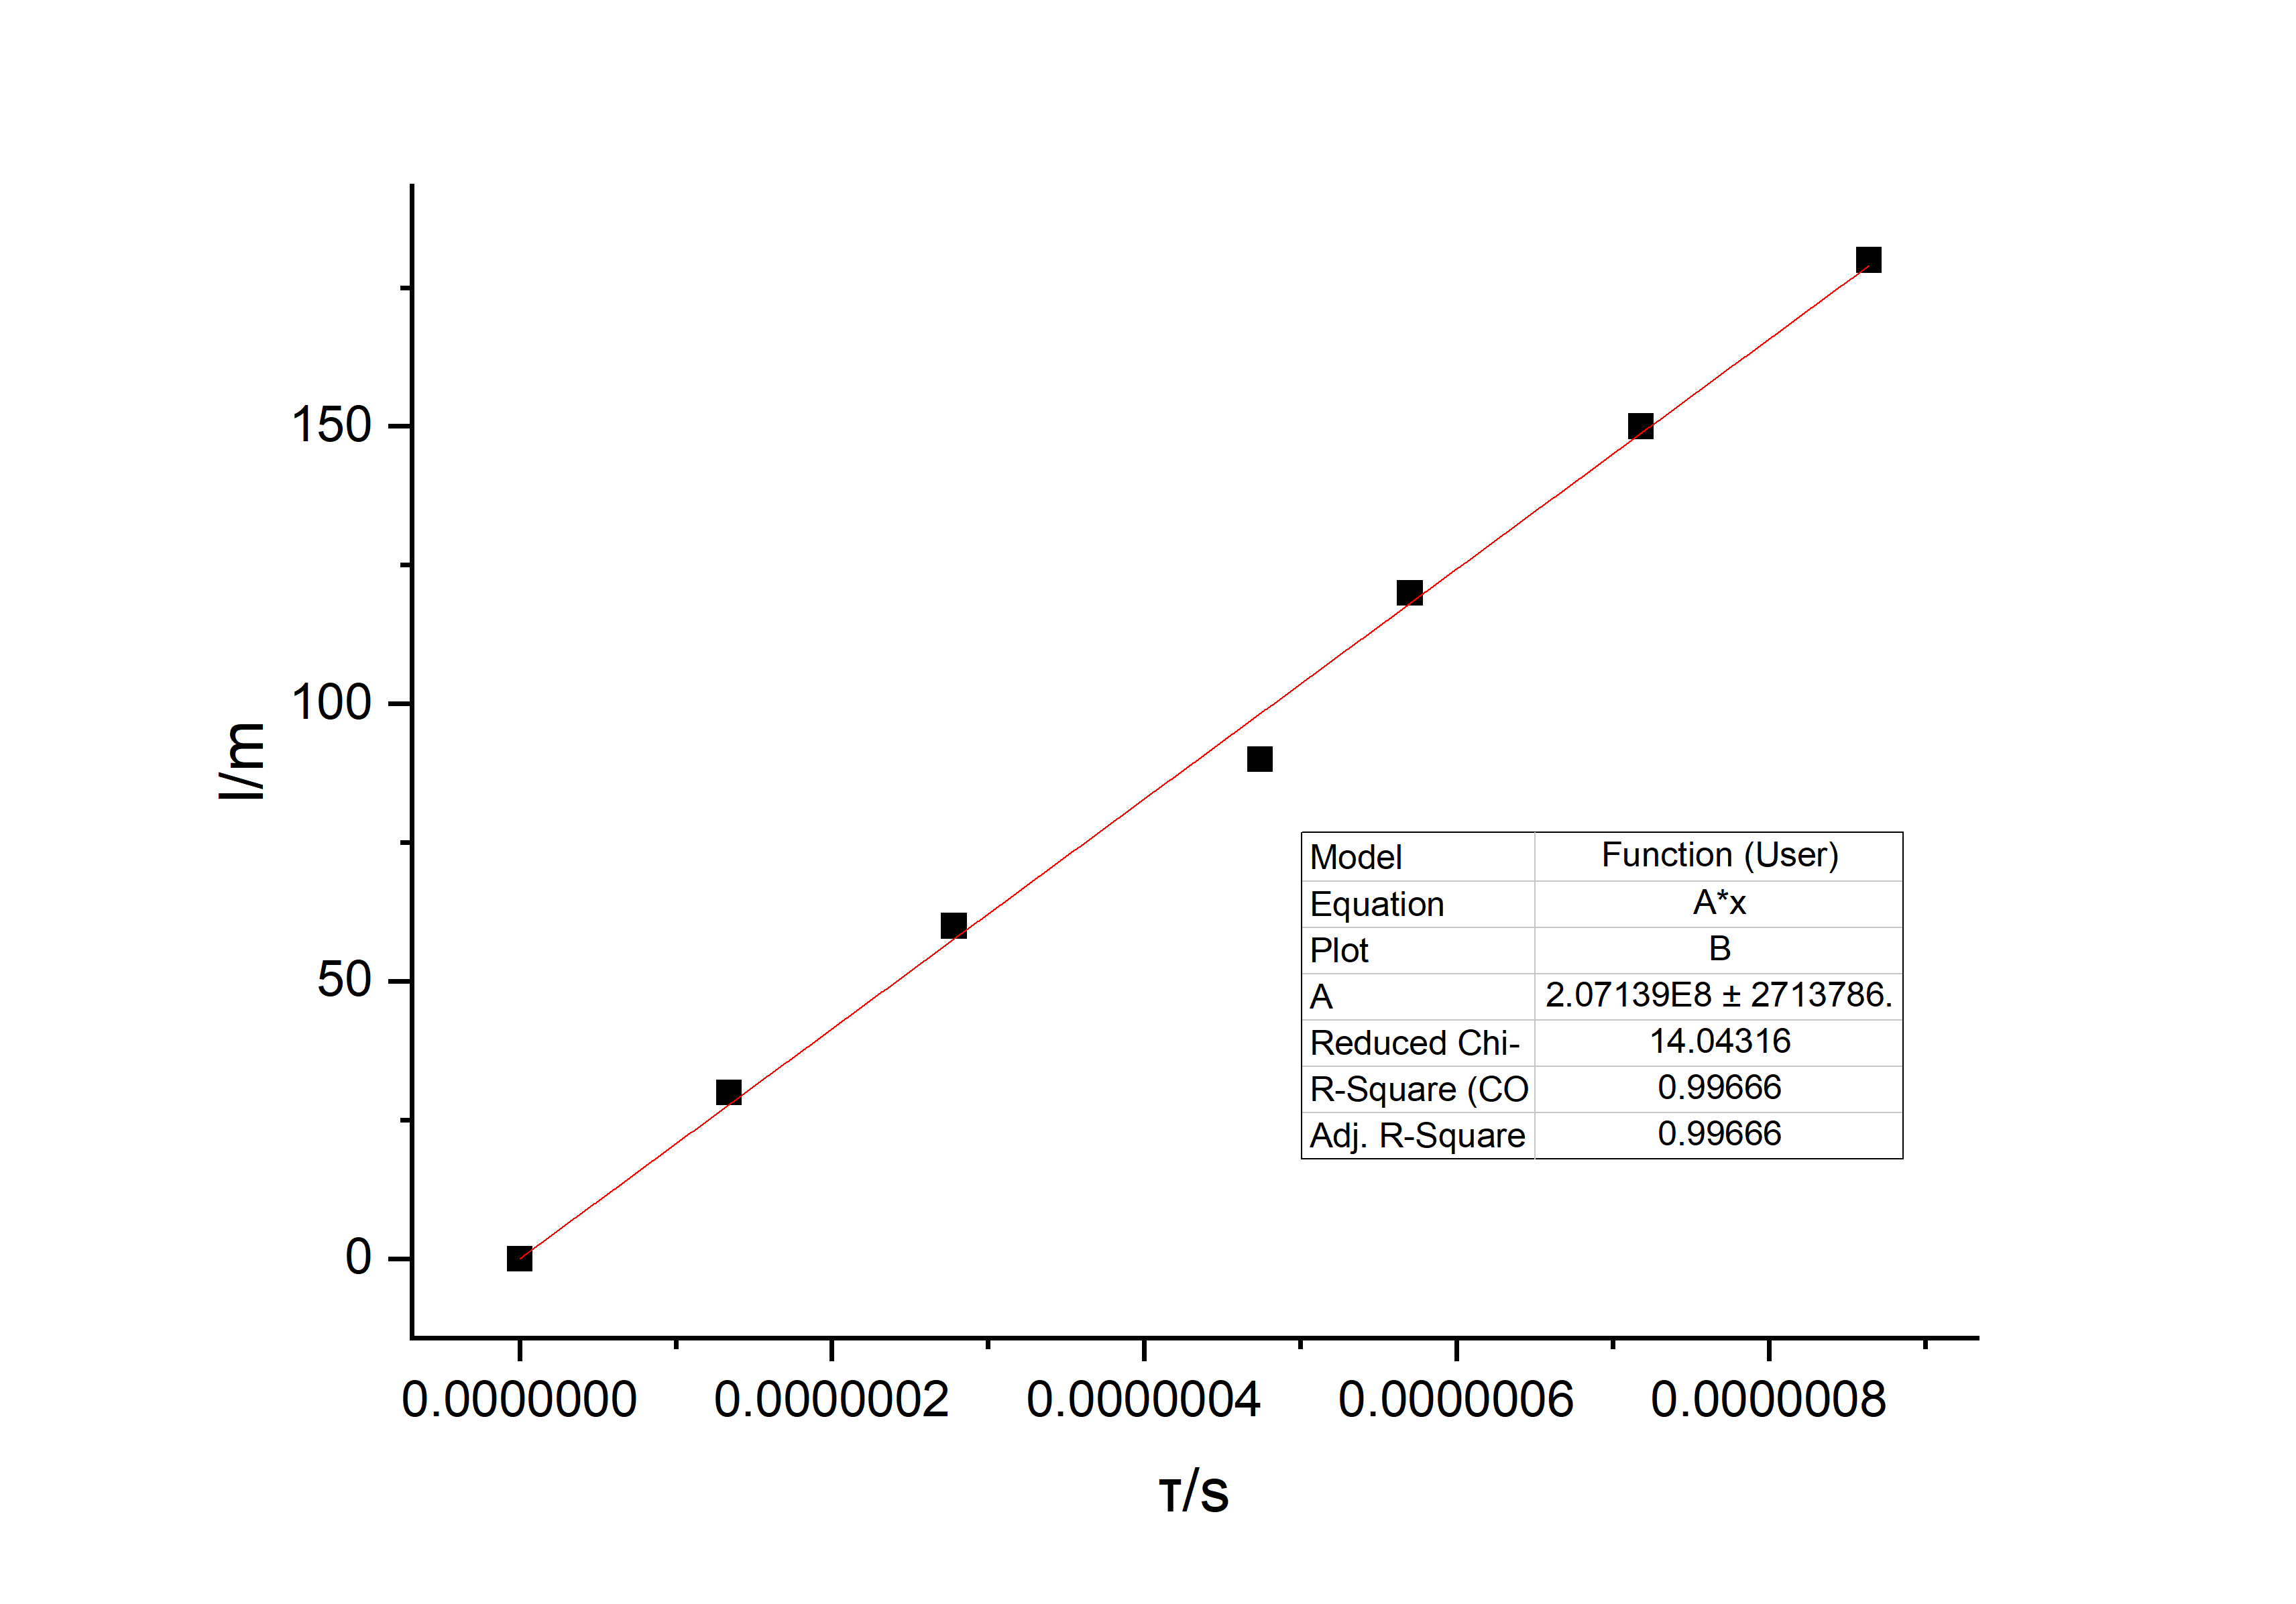
\includegraphics[scale=0.5]{linear2.png}
    \caption*{$v_p$拟合图像}     
\end{figure}
可以看到$R^2=0.99666$,可见拟合情况较好. 我们得到斜率为$k=2.071\times 10^8m/s$,即相速度为$v_p\approx2.071\times 10^8m/s$。这与 B.1 中的结果$v_p=1.974\times 10^8m/s$吻合得很好.

\subsection*{4. B.3输出功率的另一种测量方式}
在 B.3 中。我们用类似焦耳定律的方式计算了功率,下面给出一种基于能量存储与传递的观点. 

考虑长度为$\Delta z$的一小段传输线,该部分仍然可等效为一段电容与电感. 能量不断向+z方向传播,根据电容能量公式求能量密度:
\begin{equation}
    \frac{\Delta E}{\Delta z}=\frac{1}{2}CU_{max}^2
\end{equation}
则功率为:
\begin{equation}
    \frac{\Delta E}{\Delta z}v=\frac{1}{2}CU_{max}^2/\sqrt{LC}=\frac{1}{2}U_{max}^2/Z_0
\end{equation}
即得到了与 B.3 相同的表达式.

同理,利用电感能量公式计算:
\begin{equation}
    \frac{\Delta E}{\Delta z}v=\frac{1}{2}LI_{max}^2v=\frac{1}{2}(U_{max}/\sqrt{\frac{L}{C}})^2/\sqrt{LC}=\frac{1}{2}U_{max}^2/Z_0
\end{equation}
也得到了相同的答案.

\subsection*{5. 关于本实验中信号发生器波形选择的一些思考}
\paragraph{A部分} A部分我们测量了同轴电缆的电容和电感,由于电容和电感在正弦交流电下方能表现为容抗$1/i\omega C$和感抗$\omega L$,因此我们采用正弦交流信号,通过各元件分压比来计算电容和电感.
\paragraph{B部分} B部分计算了信号发生器对外输出功率,我们讨论峰峰值、有效值、功率以及阻抗时也是相对于正弦交流电而言的,因此这里采用的也是正弦交流电.
\paragraph{C部分} C部分我们通过示波器观察入射信号和反射信号,如果信号是正弦波,则各个正弦波叠加在一起,结果就无法直观观察了. 在这里我们采用脉冲信号,由于存在一定的占空比且信号没有负值,这样就保证了:i)各个峰是分立的,可以将各个入射信号和反射信号分离开,且可以直观观测到多次反射的信号;ii)对于半波损失的观察也更为直观;考虑到半波损失会导致信号振幅为负,直接观察负峰的存在与否就可以直观发现是否有半波损失.
\paragraph{D部分}D部分观察驻波,考虑到一般意义上驻波的是由频率相同、传输方向相反的正弦波形成的,因此在此处我们仍需要用正弦波信号.

\subsection*{6. 误差分析}

\textbf{i.)}示波器显示的测量值有一定误差,考虑到示波器测量时,示数会发生跳动,因此示波器测量肯定会存在一定的误差. 同时示波器内部有阻抗,测量时也会产生系统误差,虽然令$V\approx V_{R'}$可以在一定程度上消除,但仍不可避免地产生误差.\par

\textbf{ii.)}信号发生器发出的波形可能存在瑕疵,同时显示的频率也未必是实际频率,考虑到信号发生器也存在阻抗,因此以上因素均会对发出的信号产生影响.

\textbf{iii.)}从根本上说,我们的传输线模型就是一种理想的近似模型,我们不但多次运用了低损耗甚至零损耗的假设,而且我们的等效电路本身就不是严格的. 再考虑到我们采用的传输线是多根连接在一起的,其中难免会产生其他的误差.

\textbf{iv.)}在C部分,我们假设了始端$1k\Omega$为无穷大电阻,假设用导线连接内外导体为短路,但实际上它们均不严格;而且我们用示波器观测波形时,采用的是连接三通接头,这就必然导致了测量点不是理想的精确点,而对于入射和反射来说,这往往就会导致信号在示波器上的偏离.

综上,实验中我们不仅理论预测会有系统误差,实验记录也会有偶然误差,因此总得来说本实验误差较大,我们如上的数据在误差范围内良好.


\section{实验结论}
本实验中,我们首先采用负载电阻分压法测得了传输线单位长度的电容与电感分别为$C_0=7.713\times10^{-11}F/m$和$L_0=3.328\times10^{-7}H/m$,分析了电力线、磁力线分布以及低集肤效应的电流表面分布;\par

之后得到了传输线等效电路模型,通过推导和计算,得到了无损耗情况下其特征阻抗$Z_0=65.68\Omega$,相速度$v_p\approx 1.974\times 10^{8}m/s$,相对介电常数$\varepsilon_r\approx 2.310$,并计算出了给定情况下信号发生器对外输出功率为0.190W,这些能量交替储存在电容和电感中;\par

然后我们研究了界面电压反射系数、阻抗匹配条件以及相位反向条件,在给予脉冲信号的情况下,我们分别使得传输线末端开路、短路、有负载,并在三种情况下通过示波器观察了入射和反射信号,并根据测量数据计算了衰减系数$\alpha\approx 0.00689m^{-1}$,并大致得出了其特性阻抗$R\approx 60\Omega$,这一测量结果与我们先前的计算结果吻合得较好;\par

最后在给予高频简谐信号情况下计算了末端开路与短路的驻波表达式和驻波频率条件,通过示波器观察到了驻波.
\par在进行本次试验过程中,我掌握了模拟示波器的使用、同轴电缆传输线电感、电容、集肤效应、等效电路模型、信号反射和形成驻波条件等知识,并进一步了解了传播常数、特征阻抗、反射系数等概念,进一步巩固了进行物理实验的步骤和基本方法. 在后续处理数据、撰写实验报告的过程中,我还进一步对交变电路、驻波、基尔霍夫方程等相关理论知识有了进一步理解,同时回顾了线性拟合、误差分析等相关知识.
\newpage
\section{原始数据}
\begin{figure}[H]\begin{center}
    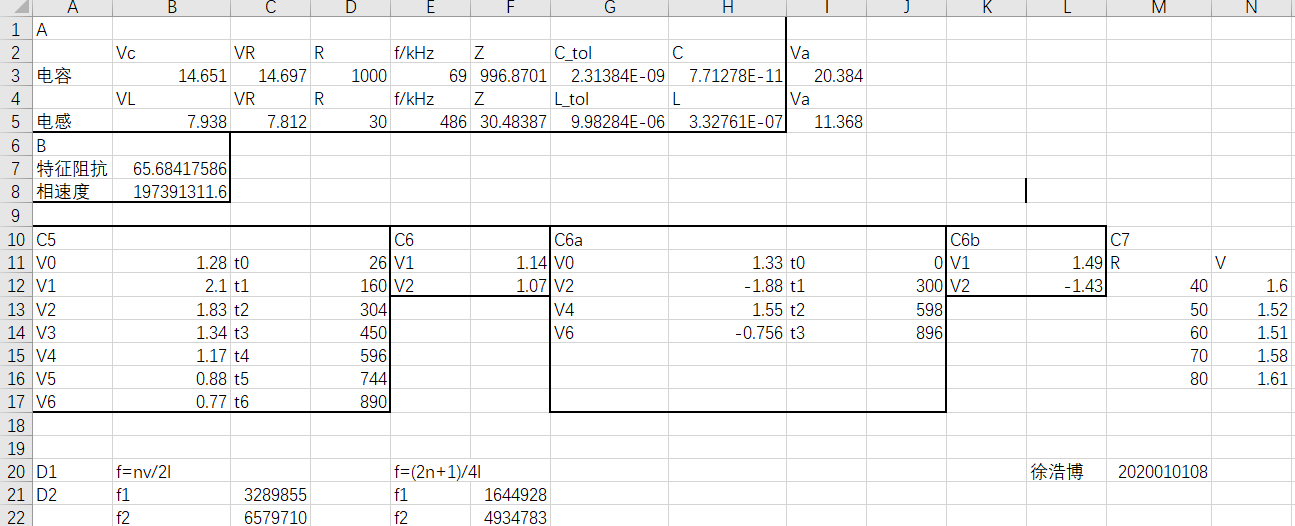
\includegraphics[scale=0.7]{data.PNG}
\end{center}\end{figure}

\end{document}

